\section{Scope and analytical design}

Agent-based modeling (ABM) explains system-level outcomes through the actions and interactions of heterogeneous agents situated in an environment. Its distinctive contribution is to make the micro-to-macro pathway explicit: agents perceive conditions, follow decision rules, interact within a network or space, and adapt or learn; their interactions can then generate patterns not specified at the aggregate level. ABM is especially useful when heterogeneity, path dependence, feedback, spatial structure, or bounded rationality is central to the research question. \footnote{Bonabeau, E. (2002). Agent-based modeling: Methods and techniques for simulating human systems. Proceedings of the National Academy of Sciences, 99(Suppl. 3), 7280–7287. https://doi.org/10.1073/pnas.082080899; Macal, C. M., \& North, M. J. (2010). Tutorial on agent-based modelling and simulation. Journal of Simulation, 4(3), 151–162. https://doi.org/10.1057/jos.2010.3; Gilbert, N., \& Troitzsch, K. G. (2005). Simulation for the social scientist (2nd ed.). Open University Press; Railsback, S. F., \& Grimm, V. (2019). Agent-based and individual-based modeling: A practical introduction (2nd ed.). Princeton University Press.}

This review draws on a corpus analysis of 29,139 publications dated 1972–2025. Titles and abstracts were classified by application domain, modeled entity, LLM involvement and function, authorship, and country. The analysis combined trend tests, logistic models with Benjamini–Hochberg correction, counterfactual Poisson analyses, and coauthorship community detection. The corpus should therefore be understood as the empirical basis for this review, not as an exhaustive census of every ABM publication. LLM findings in particular are early-diffusion estimates: the post-release observation window covers only 2023–2025. Records were collected from Web of Science, PubMed, and DBLP, deduplicated, and, where possible, enriched with abstracts through OpenAlex. \footnote{Priem, J., Piwowar, H., \& Orr, R. (2022). OpenAlex: A fully-open index of scholarly works, authors, venues, and concepts. arXiv:2205.01833. https://doi.org/10.48550/arXiv.2205.01833} The cleaning workflow excluded records that still lacked abstracts after enrichment, non-research publication types (including editorials, correspondence, and reviews), and non-English publications. The resulting strict corpus contains 29,139 publications through 2025; the broader all-years corpus contains more than 31,000 records. Figure 1 summarizes the collection and filtering process.

Figure 1 distinguishes the all-years record pool from the publication-year cutoff used in the analyses, making the corpus construction and reporting window explicit.

\begin{figure}[htbp]
\centering
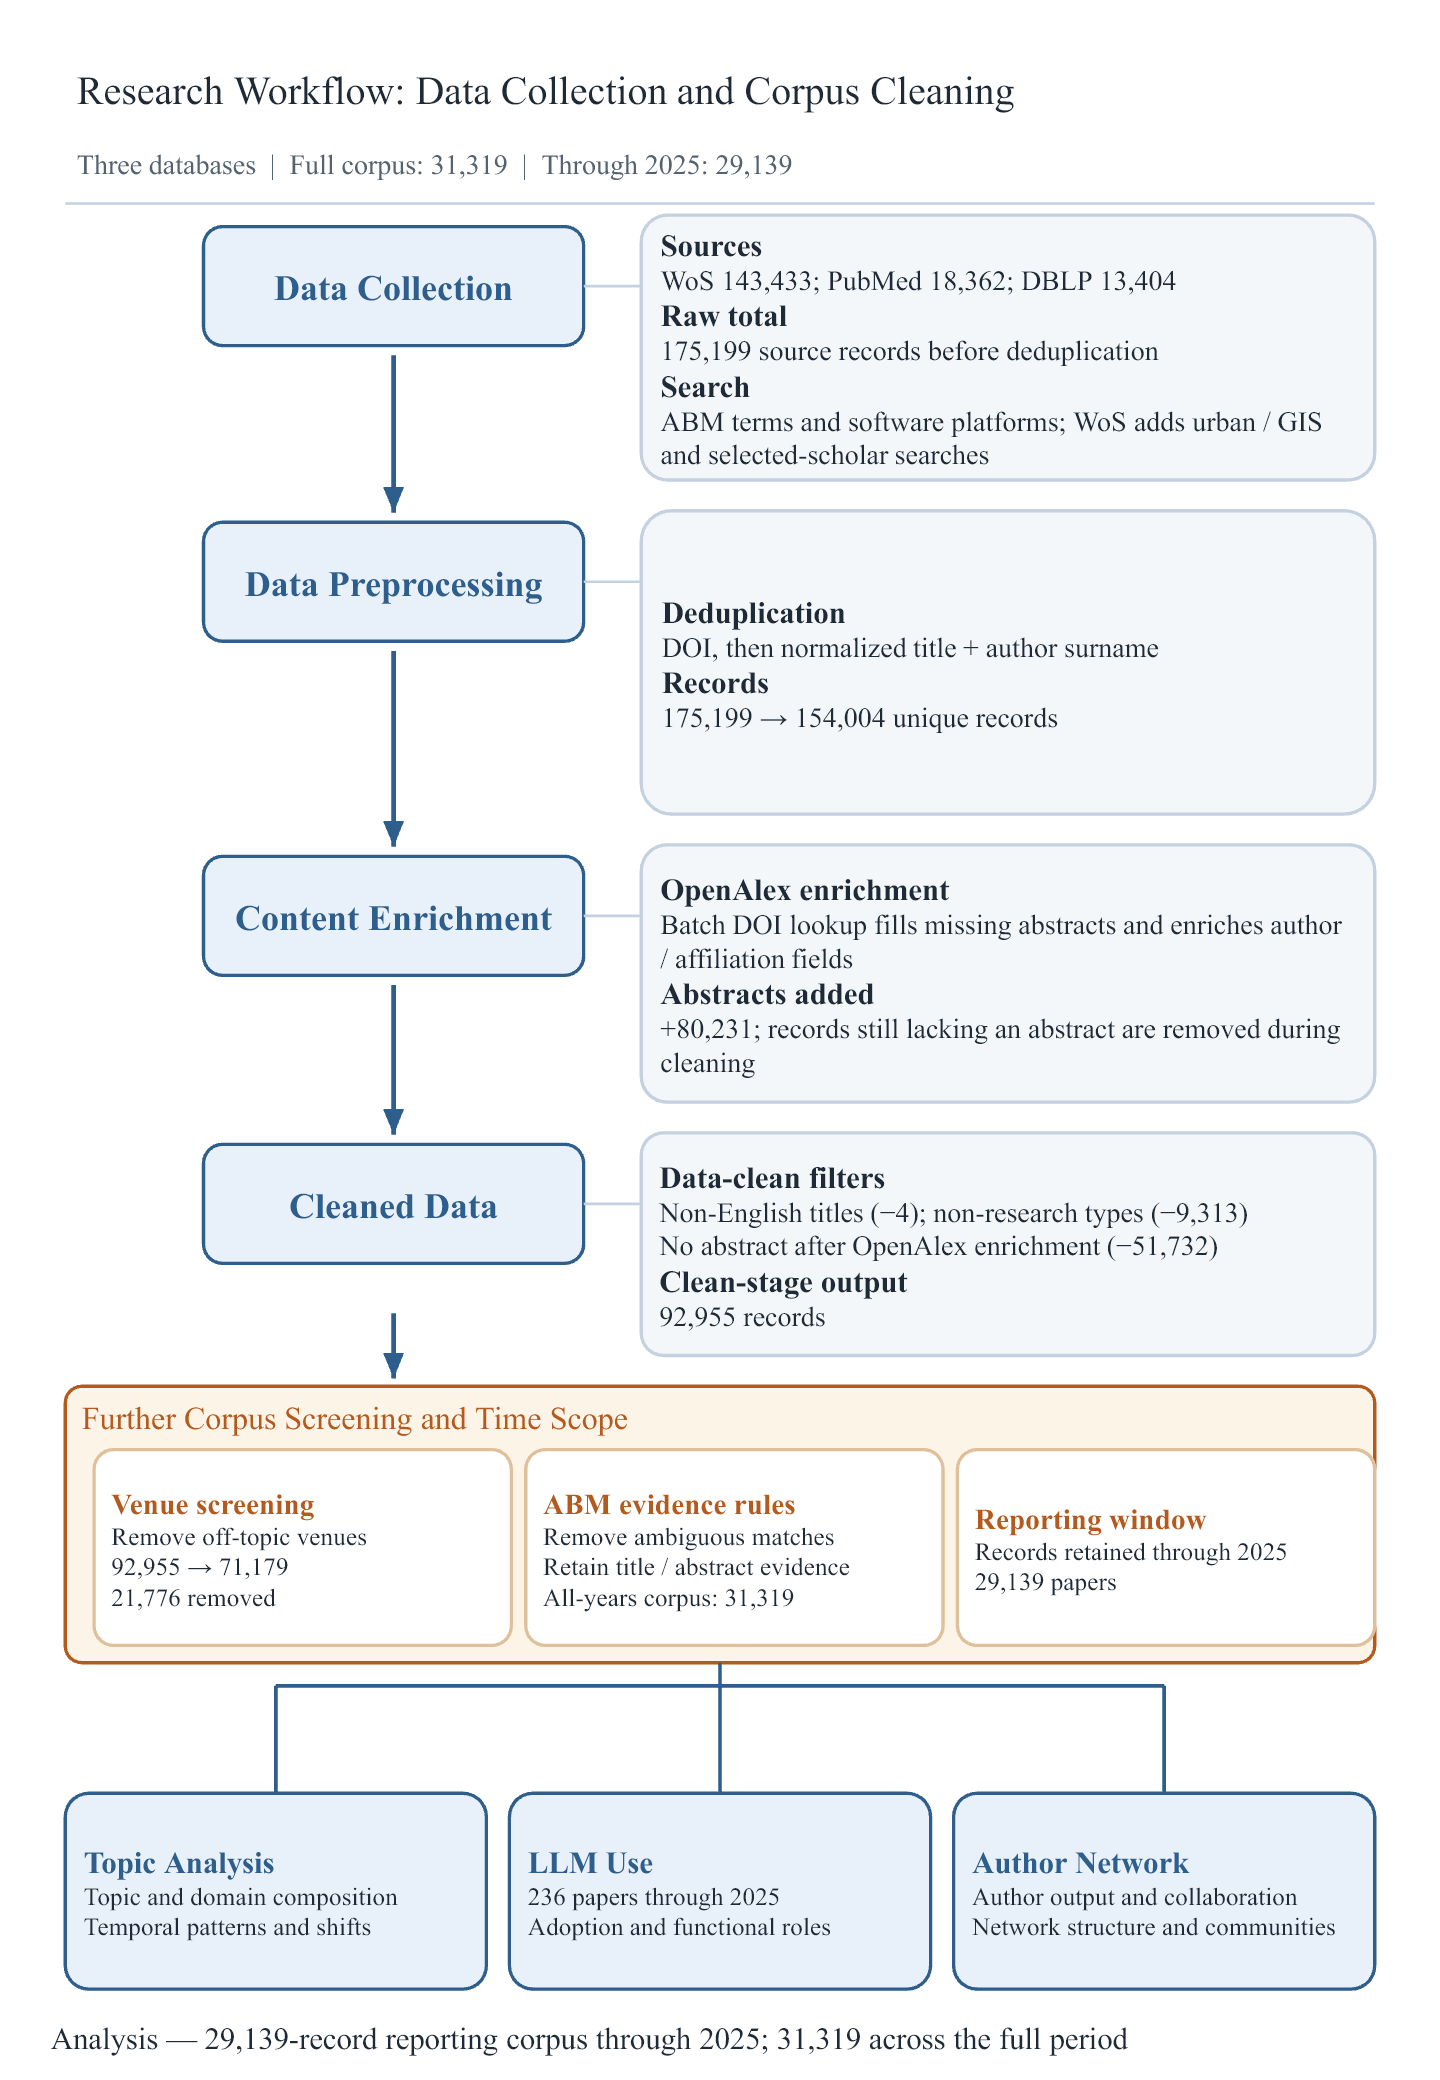
\includegraphics[width=0.88\textwidth,height=0.78\textheight,keepaspectratio]{figures/figure_01.png}
\setcounter{figure}{0}
\caption{Literature collection, abstract enrichment, data cleaning, and derivation of the analytical corpus.}
\label{fig:figure1}
\end{figure}

\begin{table}[htbp]
\centering
\small
\setlength{\tabcolsep}{3pt}
\renewcommand{\arraystretch}{1.18}
\setcounter{table}{0}
\caption{Source of collected papers}
\label{tab:table1}
\begin{tabularx}{\linewidth}{>{\raggedright\arraybackslash}p{0.27\linewidth} >{\centering\arraybackslash}p{0.12\linewidth} X}
\toprule
\textbf{Processing Stage} & \textbf{Number} & \textbf{Description} \\
\midrule
Corpus Collection & 29,139 & — \\
Web of Science & 26,307 & 15,130 papers are indexed exclusively by Web of Science \\
PubMed & 9,671 & 607 papers are indexed exclusively by PubMed \\
DBLP & 4,640 & 2,201 papers are indexed exclusively by DBLP \\
Overlapping Records Across Databases & 11,201 & Papers indexed by two or more databases; therefore, the sum of database-specific counts exceeds the total corpus size \\
Papers Using Large Language Models & 236 & As of 2025 \\
\bottomrule
\end{tabularx}
\end{table}

\subsection{DeepSeek API classification and prompt design}

Corpus-level classification used the DeepSeek API through an OpenAI-compatible asynchronous client and the deepseek-chat model. Each request included a paper’s title and abstract; abstracts were truncated at 6,000 characters, and records without an abstract were not submitted for classification. Requests used temperature 0, JSON-object output, and a 512-token response limit. The asynchronous run used checkpoints and retried eligible failures, allowing processing to resume without replacing completed results.

The classification prompt was structured as follows:

\begin{itemize}[leftmargin=1.6em,itemsep=2pt,topsep=3pt]

\item \textbf{Role:} Act as a classifier of literature on agent-based modeling (ABM) and complex systems.

\item \textbf{Evidence:} Use only information stated in the title and abstract; do not infer unsupported details.

\item \textbf{Classification fields:} Assign one primary topic, one dominant simulated-agent type, whether an LLM is used, and—if applicable—the LLM’s functional role, using the supplied standardized taxonomies.

\item \textbf{LLM-use criteria:} Count LLM use only when the model contributes to the research method. Do not count background mentions or use limited to writing, editing, translation, or literature searching. Do not treat conventional machine-learning or NLP methods as LLMs by default.

\item \textbf{Agent-type distinction:} Assign the LLM-agent category only when an LLM is part of the simulated agent architecture; distinguish this from using an LLM to support other research tasks.

\item \textbf{Output format:} Return a compact JSON object with the specified fields and taxonomy codes, without additional prose or formatting.

\end{itemize}

The returned JSON was parsed and checked before being merged with the corpus. This constrained design improves consistency and auditability, but it does not remove classification uncertainty or the need for human validation.